% Original source and additional resources is available on:
% https://github.com/janusvm/aau-maok-p1

\documentclass[12pt,a4paper,oneside,final]{article}

% PREAMBLE ---------------------------------------------------------------------
\title{
  Vejledning p{\aa} P1\\
  Matematik-{\O}konomi
}
\author{
  Janus Valberg-Madsen \href{mailto:janus@math.aau.dk}{\texttt{<janus@math.aau.dk>}}\\
  vejleder for grupperne XXXX og YYYY
}
\date{14.\ oktober 2019}

% Packages
\usepackage[T1]{fontenc}
\usepackage[utf8]{inputenc}
\usepackage[danish]{babel}
\usepackage[danish]{translator}
\usepackage{hyperref}
\usepackage[charter]{mathdesign}
\usepackage{inconsolata}
\usepackage[labelfont=bf,font=it]{caption}
\usepackage[margin=2.5cm]{geometry}
\usepackage[shortlabels]{enumitem}
\usepackage[dvipsnames]{xcolor}
\usepackage{graphicx}
\usepackage{tikz}
\usepackage{mathtools}
\usepackage{bbm}
\usepackage{bm}


% Commands
\newcommand{\N}{\mathbb{N}}
\newcommand{\Z}{\mathbb{Z}}
\newcommand{\R}{\mathbb{R}}
\newcommand{\1}{\mathbbm{1}}
\newcommand{\e}{\mathrm{e}}
\newcommand{\vzero}{\bm{0}}
\newcommand{\vx}{\bm{x}}
\newcommand{\vb}{\bm{b}}
\newcommand{\vc}{\bm{c}}
\newcommand{\vs}{\bm{s}}
\newcommand{\nodemark}[1]{\tikz[baseline=-0.5ex]\node[#1] at (0,0) {};}


% Settings
\setlist{itemsep=0pt}
\usetikzlibrary{arrows.meta,backgrounds,calc,calendar,positioning}
\tikzstyle{afternoon} = [shape=rectangle,minimum size=1.5em,fill=SkyBlue]
\tikzstyle{morning}   = [shape=rectangle,minimum size=1.5em,fill=Lavender]
\tikzstyle{special}   = [shape=rectangle,minimum size=1.5em,fill=YellowGreen]
\tikzstyle{asym}      = [shape=rectangle,minimum size=1.0em,fill=SkyBlue]
\tikzstyle{msym}      = [shape=rectangle,minimum size=1.0em,fill=Lavender]
\tikzstyle{ssym}      = [shape=rectangle,minimum size=1.0em,fill=YellowGreen]
\tikzstyle{point}     = [text=white,fill,shape=circle,minimum size=5pt,inner sep=0pt]



% MAIN -------------------------------------------------------------------------
\begin{document}
\maketitle

\renewcommand{\abstractname}{Om dette dokument}
\begin{abstract}
  Dette dokument beskriver mine forventninger for, hvordan samspillet mellem vejleder og projektgruppe skal foregå på første studieår for Matematik-Økonomi.
  En oversigt gives over, hvad de studerende skal gøre forud for og under vejledermøder, hvornår sådanne møder kan forekomme, og hvilke former for hjælp, jeg kan yde.
\end{abstract}


\section{Vejledermøder}
\subsection{Tidspunkter}
\label{subsec:tidspunkter}
Der er mulighed for at have op til \textbf{\'et vejledermøde \`a højst halvanden time om ugen}, og I kan vælge imellem de markederede dage i kalenderen nedenfor:
\begin{center}
  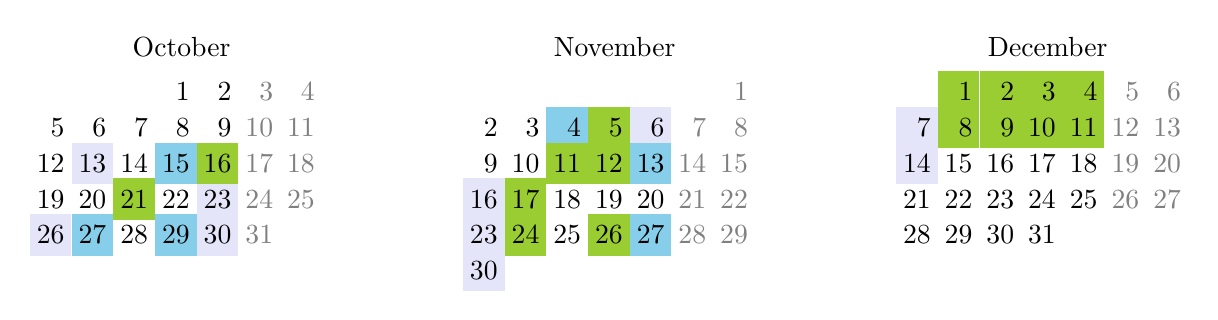
\begin{tikzpicture}[every calendar/.style={week list,month label above centered,day text={\%d=}}]
  \calendar (oct) [dates=2020-10-01 to 2020-10-last] at (0,0) if (weekend) [Gray];
  \calendar (nov) [dates=2020-11-01 to 2020-11-last] at (5.5,0) if (weekend) [Gray];
  \calendar (dec) [dates=2020-12-01 to 2020-12-last] at (11,0) if (weekend) [Gray];

  % Available dates
  \begin{scope}[on background layer]
    % October
    \foreach \d in {13,23,26,30} \node[morning] at (oct-2020-10-\d) {};
    \foreach \d in {15,27,29} \node[afternoon] at (oct-2020-10-\d) {};
    \foreach \d in {16,21} \node[special] at (oct-2020-10-\d) {};
    % November
    \foreach \d in {06,16,23,30} \node[morning] at (nov-2020-11-\d) {};
    \foreach \d in {04,13,27} \node[afternoon] at (nov-2020-11-\d) {};
    \foreach \d in {05,11,12,17,24,26} \node[special] at (nov-2020-11-\d) {};
    % December
    \foreach \d in {07,14} \node[morning] at (dec-2020-12-\d) {};
    \foreach \d in {01,02,03,04,08,09,10,11} \node[special] at (dec-2020-12-\d) {};
  \end{scope}
\end{tikzpicture}

\end{center}
hvor
\begin{itemize}[label={},wide,labelindent=0pt,topsep=1ex]
\item \nodemark{msym} angiver dage, hvor jeg er tilgængelig \textbf{om formiddagen (9:00--12:00)}
\item \nodemark{asym} angiver dage, hvor jeg er tilgængelig \textbf{om eftermiddagen (12:30--15:30)}
\item \nodemark{ssym} angiver dage, hvor jeg er tilgængelig \textbf{kun hvis \emph{begge} mine grupper ønsker at have et møde den pågældende dag}.
  Dette skyldes at jeg disse dage ikke har andre ærinder på Basis, så jeg ville skulle tage derud udelukkende for at holde vejledermøder.
\end{itemize}

\clearpage
\subsection{Booking af møder}
\label{subsec:booking}
Det er op til jer at indkalde til vejledermøder, når I har brug for dem.
Mødeindkaldelser skal ske via kalenderinvitation på \url{https://mail.aau.dk}:
\begin{enumerate}[itemsep=0pt]
\item Opret et møde på en dag, hvor jeg er tilgængelig (ifølge Afsnit \ref{subsec:tidspunkter})
\item Tilføj mig (\texttt{janus@math.aau.dk}) og alle gruppemedlemmer som mødedeltagere
\item Vælg et tidsinterval på op til 1½ time, sådan at det stadig er muligt for mig at holde et møde samme dag med den anden gruppe, hvis de ønsker det
\item Vedhæft arbejdsblade i PDF-format, og skriv læsevejledningen til dem ind i mødebeskrivelsen (se Afsnit \ref{sec:arbejdsblade} for en uddybelse af dette)
\item Skriv dagsordenen og spørgsmål ind i mødebeskrivelsen
\item Angiv jeres grupperum i lokale-feltet
\end{enumerate}
Indkaldelsen (med arbejdsblade og alle de nævnte informationer) skal være afsendt \textbf{senest kl.\ 16 to dage før den ønskede mødedag} for at sikre, at jeg har en chance for at nå at læse arbejdsbladene.
Hvis mødet ligger om mandagen, vil jeg dog kræve, at indkaldelsen foreligger allerede \textbf{fredag kl.\ 16}.

Ønsker I et vejledermøde på en \nodemark{ssym}-dag, skal møderne for begge grupper ligge i forlængelse af hinanden.
Sørg i alle tilfælde for at koordinere mødetider med den anden gruppe.

\subsection{Dagsorden}
Alle mødeindkaldelser skal indeholde en dagsorden for mødet.
I kan med fordel bruge følgende liste som en skabelon for, hvad en sådan dagsorden kunne indeholde:
\begin{enumerate}[itemsep=0pt]
\item Mødets formål (hvad mødes vi for?)
\item Status på gruppearbejdet (hvad har I hver især lavet siden sidst, hvordan fungerer gruppearbejdet, har I haft nogle problemer, overholder I tidsplanen, etc.)
\item Svar på spørgsmål (hvis I har angivet dem i mødeindkaldelsen)
\item Kommentarer til arbejdsbladene (hvis I har vedhæftet dem i mødeindkaldelsen)
\item Plan for næste uge (hvad skal I lave indtil næste gang vi ses?)
\item Eventuelt (andre ting, som I gerne vil have vendt med mig)
\item Evaluering af mødet (blev mødets formål opfyldt?)
\end{enumerate}
Der må selvfølgelig gerne være flere punkter, men jeg vil anbefale, at I altid som minimum har de ovenstående med, så I får så meget ud af møderne som muligt.

\subsection{Referat}
\'En af gruppemedlemmerne skal tage referat af vejledermødet, som efter mødet sendes til hele gruppen og mig via email.
Undgå venligst at vedhæfte referatet som fil, men skriv istedet indholdet direkte ind i emailen (dette gør det bl.a.\ lettere at søge i referater senere).


\clearpage
\section{Arbejdsblade}
\label{sec:arbejdsblade}
Med \emph{arbejdsblade} menes der en kompileret PDF-fil med seneste, gennemrettede udgave af hele jeres projekt, og en \emph{læsevejledning} hertil er en liste over de afsnit/sider, som I gerne vil gerne have jeg kigger på, samt begrundelser herfor.
Vær opmærksom på, at:
\begin{itemize}
\item alle afsnit, som jeg skal læse, skal være så gennemarbejdede som muligt og gennemlæst af hele gruppen---inkl.\ for stave- og grammatikfejl
\item jo flere afsnit I skriver i læsevejledningen, jo mere overfladisk bliver min læsning
\item jeg kun læser samme afsnit to gange, hvis der er sket meget markante ændringer
\item arbejdsblade sendt uden læsevejledning eller efter deadline (se Afsnit \ref{subsec:booking}) ikke læses
\end{itemize}

\section{Hvad jeg kan hjælpe med}
Foruden det faglige indhold i rapporten og det organisatoriske i arbejdsprocessen, kan jeg også hjælpe med tekniske ting omkring
\begin{itemize}
\item \LaTeX{} og dokument-/projektstruktur
\item Git og GitHub
\item Programmering i Julia, R eller Python
\end{itemize}
Jeg hjælper \emph{ikke} med: Overleaf, Microsoft Office, Dropbox/Google Drive/OneDrive, Maple, MATLAB, eller andre proprietære CAS-værktøjer.
I må selvfølgelig stadig godt bruge dem, blot I ikke forventer, at jeg kan svare på spørgsmål eller løse problemer, der involverer dem.

\subsection{Kommentarer via GitHub}
Hvis I har jeres projekt under versionsstyring på \href{https://github.com}{GitHub} kan I invitere mig som \emph{Collaborator} (brugernavn: \href{https://github.com/janusvm}{\texttt{janusvm}}).
Så vil jeg kunne kommentere direkte på kode, oprette/deltage i Issues, og have adgang til seneste version af jeres projekt.
Dette kan gøre det nemmere for mig at hjælpe jer, hvis I f.eks.\ har problemer med \LaTeX{} eller Julia/R/Python og har brug for hjælp til fejlfinding.

Brugen af Git og GitHub er ikke et krav, men det er en stor fordel for jer at kende til.
I det omgang, I skulle ønske det, har jeg mulighed for at hjælpe jer i gang med et GitHub-baseret workflow.

\section{Kontakt}
Hvis I har spørgsmål om småting, som ikke kan vente til næste vejledermøde, kan I kontakte mig på email.
Jeg læser emails regelmæssigt inden for normal arbejdstid og bestræber mig på at svare hurtigst muligt.

Alle emails til mig skal have hele gruppen på CC, så alle kan følge med i samtalerne.
Sørg af denne grund for at trykke \emph{Svar til alle}, når I besvarer emails fra mig.
Derudover må I meget gerne underskrive alle emails med jeres gruppenummer, så jeg lettere kan holde styr på de forskellige grupper.

Husk i øvrigt at tjekke jeres emails regelmæssigt.

\end{document}

%%% Local Variables:
%%% mode: latex
%%% TeX-master: t
%%% End:
